\section{Harness Details}
\label{app:harness}

\subsection{Agent loop}
\label{app:tool-loop}

Each episode runs one paper with one model, opening with a fixed system
message and a task prompt rendered from the paper's dataset row
(Appendix~\ref{app:prompts}), and every request includes the tools of
Appendix~\ref{app:toolset} and an ephemeral status line giving the rounds used and
remaining. A turn may issue several tool calls, which the harness executes in
order, appending one truncated JSON result each, and
Figure~\ref{fig:app-a-round-anatomy} shows one round as the event
transcript records it. Near the served context
window a compaction step elides older tool results, leaving a placeholder with
the character count and the on-disk path of the elided text. An episode ends
when the model returns no tool call, reaches the round cap, exhausts its
compute budget, overflows the context beyond what elision relieves, or hits an
unrecoverable error, and the harness then issues one final tool-free request
constrained to the report schema of Appendix~\ref{app:report-format}.
The launch scripts of Appendix~\ref{app:models} record the values a sweep
set.

\begin{figure}[htb]
\centering
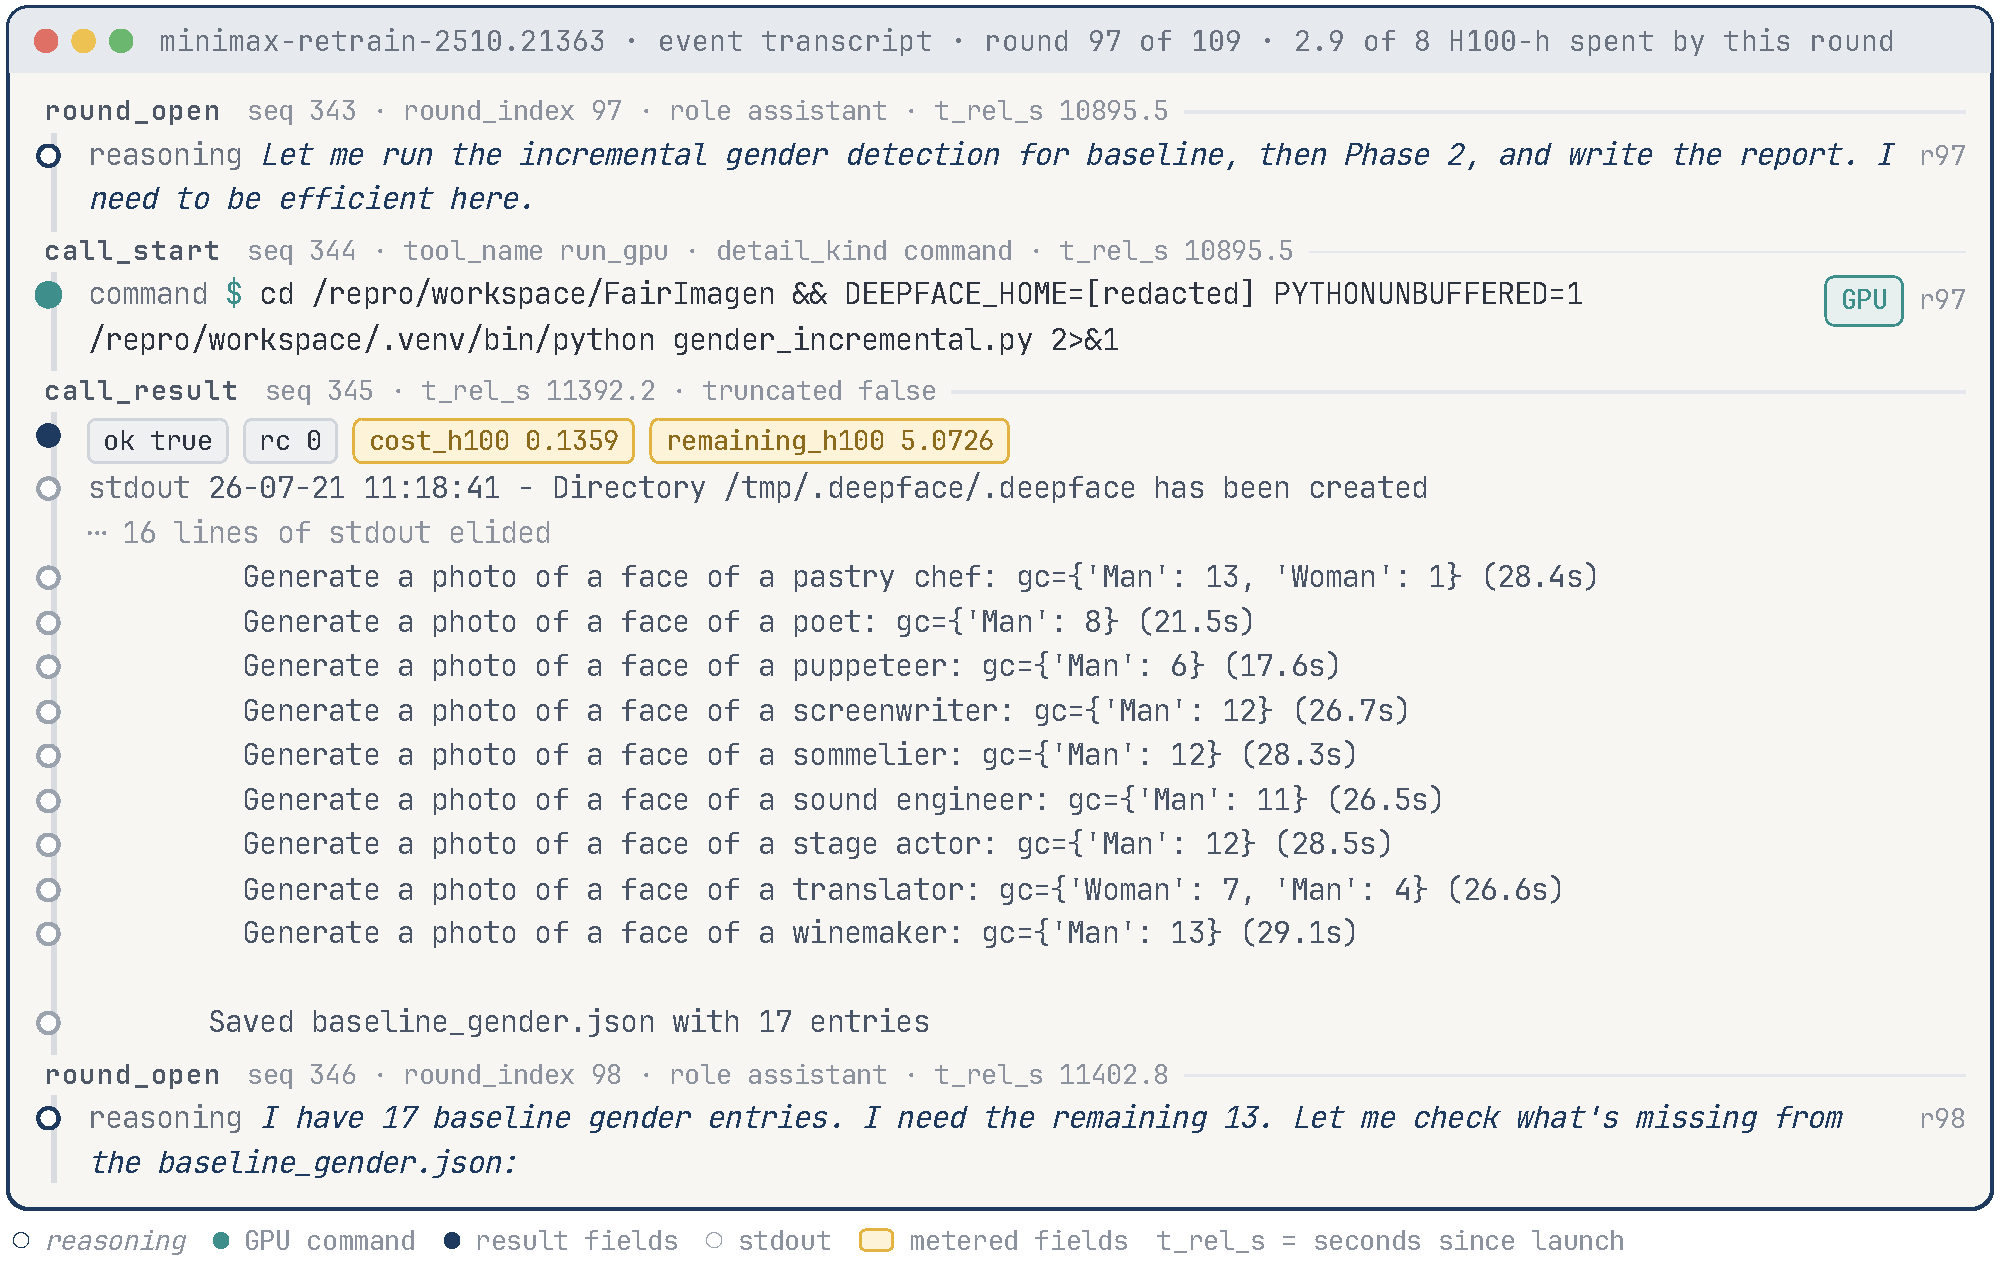
\includegraphics[width=\textwidth]{figures/app_A_round_anatomy}
\caption{Round 97 of MiniMax-M2.7 on FairImagen~\citep{fu2025fairimagen} as the
event transcript records it, from the reasoning to the metered
\texttt{run\_gpu} result.}
\label{fig:app-a-round-anatomy}
\end{figure}

\subsection{Tools}
\label{app:toolset}

The model acts through the seven tools of Table~\ref{tab:tools}, and because
there is no file-reading tool and no general web search, it reads files through
the shell with \texttt{grep}, \texttt{sed}, and \texttt{cat} and can fetch only
URLs it already knows or can construct. We granted one exception in the task
prompt, a third-party library-documentation search at \texttt{context7.com} the
model may query through \texttt{fetch\_url}, and since no harness code path
depends on that service, a failed fetch returns an error and the episode
continues.

\begin{table}[ht]
\centering
\small
\renewcommand{\arraystretch}{1.15}
\begin{tabular}{@{}l>{\raggedright\arraybackslash}p{9.4cm}@{}}
\toprule
Tool & Function \\
\midrule
\texttt{workspace\_bash} & Bash with the episode workspace as the working
directory, on the node that runs the harness, with no GPU passed through.
Cloning, installs, edits, inspection. Timeout default 900\,s, maximum
3{,}600\,s. Returns stdout, stderr, exit code, and duration. \\
\texttt{write\_file} & Write a UTF-8 file under the workspace or evidence roots,
up to 200{,}000 characters, overwriting an existing file at that path. \\
\texttt{edit\_file} & Replace one exact string in an existing file. The match
must be unique unless \texttt{replace\_all} is set. A bare repo-relative path is
located by suffix search when it resolves to exactly one file. \\
\texttt{update\_plan} & Replace the agent's ordered checklist of steps with
statuses \texttt{pending}, \texttt{in\_progress}, or \texttt{completed}. At most
one step may be \texttt{in\_progress}. \\
\texttt{fetch\_url} & Fetch a public http(s) URL and reduce HTML to text,
default 24{,}000 characters. \\
\texttt{list\_partitions} & Run \texttt{sinfo} and return each Slurm partition's
node counts by state, walltime limit, and GPU resources, plus the profile
default. Read-only. \\
\texttt{run\_gpu} & Run one command on the held GPU allocation
(Appendix~\ref{app:gpu-metering}). The only path to a GPU. \\
\bottomrule
\end{tabular}
\caption{The seven tools available to the model, with the code defaults and
caps each enforces.}
\label{tab:tools}
\end{table}

\subsection{Hardware setup and compute accounting}
\label{app:gpu-metering}

\texttt{run\_gpu} holds one Slurm allocation across calls, as
Figure~\ref{lst:slurm-lifecycle} shows, acquiring it on the first call with a
fixed GPU count and wall cap and re-acquiring near the cap. Queue time is free,
and held time is charged between rounds, idle time while the model reasons
included. The harness refuses any allocation whose worst-case cost exceeds the
remaining budget, and once the budget is exhausted it releases the session and
issues the final report turn. The meter charges GPU count times held wall clock
times a hardware multiplier, which is 1.0 for the single GH200 profile every run
used, so the per-hardware figures the task prompt prints guide the agent's
planning and never enter the charge.

\begin{codebox}[lst:slurm-lifecycle]{bash}{Allocation lifecycle}
# acquire once; returns the instant the allocation is granted, then stays up
$ salloc --no-shell -A <account> -p <partition> --nodes=1 \
      --gpus=<k> --mem=<100*k>G --cpus-per-gpu=60 --time=<minutes>
# run each step into the held jobid, with no new queue wait
$ srun --jobid=<jobid> --ntasks=1 --unbuffered \
      apptainer exec --nv ... <image> bash -lc 'cd /repro/workspace && <cmd>'
# release when the agent is done, or at episode teardown
$ scancel <jobid>
\end{codebox}

\subsection{Environment details}
\label{app:sandbox}

Every shell step runs inside an Apptainer
container~\citep{kurtzer2017singularity} whose image is a read-only CUDA 12.9
and cuDNN development root with git, a C and C++ build chain, \texttt{uv}, and
Python 3.12 but no preinstalled PyTorch, and since that image is aarch64 like the
GH200 Grace hosts, every dependency the agent installs needs an aarch64 wheel or
a source build. Only bound paths are visible, the
workspace and evidence directories read-write at \texttt{/repro/workspace} and
\texttt{/repro/evidence}, the paper's reference copy read-only at
\texttt{/repro/reference}, and node-local \texttt{/tmp} and the shared package
caches read-write. The host home is not mounted.

\subsection{Run bundle and report format}
\label{app:report-format}

Each run writes a self-contained run bundle at
\texttt{<runs-dir>/\allowbreak<arxiv\_id>/\allowbreak<budget>h/\allowbreak<run\_id>/}.
The writable \texttt{workspace/} holds the agent's clones and scripts. The
read-only \texttt{reference/} holds the paper's LaTeX sources, its OpenReview
supplement, a file manifest, and an \texttt{info.json} of IDs. The
\texttt{evidence/} directory holds four fixed entries (\texttt{commands.log},
\texttt{trajectory.jsonl}, \texttt{env.lock}, and \texttt{patches/}), plus
one numbered log per GPU step, \texttt{plan.md}, and the \texttt{REPORT.md}
the task prompt requires. Per-run token counts and GPU-utilization samples are
recorded alongside. For the runs in this paper we bound \texttt{evidence/}
read-write, so the agent could rewrite the harness-written
\texttt{commands.log} and \texttt{trajectory.jsonl}, and the harness checked
neither file while a run was live. The auditor traces every number to the
command that produced it. Because the agent could edit these two files, we
compared every logged entry with the transcript the harness writes on the
host, outside the sandbox.

\paragraph{Log comparison.} For each of the 372 graded runs we matched every
entry that an agent command produced in the two files against the host
transcript, requiring the same command and return code and, for
\texttt{run\_gpu} entries, the same cost and remaining budget.
Table~\ref{tab:log-check} gives the outcome for the 45,861 such entries, and
the other 3,724 rows of the two files are written by the harness itself. We
also searched every agent command for writes to the two files. One run wrote
to \texttt{commands.log}, where MiniMax-M2.7 on 2510.25146 replaced the file
with its own notes through a \texttt{write\_file} call, and the auditor had
graded that run 1 of 10 as unverifiable. No run wrote to
\texttt{trajectory.jsonl}. The comparison also found 119 commands in 65 runs
that the harness ran and did not write to \texttt{commands.log}, because two
early-return paths in the harness skip the log, and the host transcript holds
all of them. The host transcript is not hash-chained, so it is not
tamper-evident by construction, and its protection is that it lies outside
every directory the sandbox mounts. The comparison detects edits made through
the agent's own commands, which the transcript records, and it detects no
other kind of edit.

\paragraph{Read-only logs.} After this comparison we changed the harness so
that the agent can no longer edit the two files. The sandbox mounts
\texttt{commands.log} and \texttt{trajectory.jsonl} read-only on top of the
read-write \texttt{evidence/} directory, and the \texttt{write\_file} and
\texttt{edit\_file} tools refuse both paths. In a test inside the sandbox,
appending to, overwriting, deleting, renaming and replacing either file all
fail, while the harness still appends to both from the host. The 372 graded
runs predate this change, and the comparison above is their check.
% src: results/e5/README.md:9-17 (372/372 matched; 45,861 of 49,585 entries checked, 3,724 host-written; 45,673 passed; 185 explained; 3 unmatched; 1 write into commands.log, run 2510.25146; 65 runs missing 119 headers, workspace_bash.py:76-77 and run_gpu.py:145); results/e5/summary.json

\begin{table}[ht]
\centering
\small
\begin{tabular}{@{}lr@{}}
\toprule
Entry & Count \\
\midrule
Matches exactly & 45,673 \\
Call refused by the harness, so no cost line & 100 \\
Remaining budget within 0.00015 H100-hours & 60 \\
First attempt of a retried call & 25 \\
Remaining budget differs by up to 0.0003 H100-hours, cost equal & 3 \\
\midrule
Total & 45,861 \\
\bottomrule
\end{tabular}
\caption{Agent-issued entries of \texttt{commands.log} and \texttt{trajectory.jsonl}
compared with the host transcript over the 372 graded runs.}
\label{tab:log-check}
\end{table}
% src: results/e5/README.md:11 and :18 (100, 60, 25 explained; 3 unmatched at 0.0002 to 0.0003 h with cost equal)

On the final, tool-free turn the model's output is constrained to a JSON
schema and saved as \texttt{report.json} beside \texttt{evidence/}, with the
fields of Table~\ref{tab:report-schema}. The harness overwrites
\texttt{paper\_id} with the ID it dispatched, so the model's echoed ID cannot
alter provenance, and records a
\texttt{report\_status} and the loop's
\texttt{exit\_reason}. Output that fails to parse or fails the structural
check is still written as a malformed report whose \texttt{report\_status} is
\texttt{degraded} and which includes the validation errors and an excerpt of
the raw output.

\begin{table}[ht]
\centering
\small
\renewcommand{\arraystretch}{1.15}
\begin{tabular}{@{}l>{\raggedright\arraybackslash}p{9.2cm}@{}}
\toprule
Field & Content \\
\midrule
\texttt{paper\_id} & The paper's arXiv ID. \\
\texttt{claim} & The claim the agent worked toward, in the agent's own words. \\
\texttt{what\_ran} & What was executed, from the environment build to
the run. \\
\texttt{scoring\_command} & One command that reproduces the measured number from
a clean state. Empty when nothing ran. \\
\texttt{measurements} & Array of measured metrics. Each entry records the metric
name with units, the observed value, the paper's reference value or
\texttt{null}, the scope the value was measured over, and an array of citations
into \texttt{evidence/} supporting the observed value. \\
\texttt{agent\_assessment} & One of \texttt{reproduced}, \texttt{partial},
\texttt{not\_reproduced}, \texttt{could\_not\_run}. \\
\texttt{changes\_made} & Deviations from the released reference. \\
\texttt{blockers} & What blocked a reproduction, empty when nothing did. \\
\texttt{evidence\_files} & The files under \texttt{evidence/} the auditor should
open first. \\
\bottomrule
\end{tabular}
\caption{The nine fields of \texttt{report.json}, all required by the schema.}
\label{tab:report-schema}
\end{table}

Once the episode finishes the harness prunes the agent's virtual environment
and any oversized files from the workspace, and the auditor grades from
\texttt{report.json} and \texttt{evidence/} (Section~\ref{sec:auditing}).

\subsection{Prompt templates}
\label{app:prompts}

Figure~\ref{lst:harness-messages} in Appendix~\ref{app:prompt-listings} prints
every fixed string the model reads: the system message stored at index 0,
where compaction never reaches it, the final-turn instruction appended once
the harness removes the tools, and the five strings inserted during an
episode. The task prompt is the first user turn, a 290-line template whose
fourteen placeholder fields under nine headings are filled from the paper's
dataset row (Appendix~\ref{app:dataset-schema}), from the episode's compute
ceiling, or from the container paths of Appendix~\ref{app:sandbox}. Rendering
fails on an unfilled field, every field has a fallback string that states
absence, and the renderer omits \texttt{match\_target.config}, so the agent
derives the configuration that produces the target value from the paper.
Figure~\ref{lst:task-prompt} prints the template.

